\documentclass[12pt,a4paper]{article}
\usepackage[UTF8]{ctex}
\usepackage{amsmath,amssymb}
\usepackage{xcolor}
\usepackage{hyperref}
\usepackage{geometry}
\usepackage{graphicx}
\geometry{margin=2.5cm}

\title{Coupling Map / 耦合映射}
\author{QuoNic}
\date{}

\begin{document}
\maketitle

\begin{center}
\textbf{Compilation / 编译} | 难度：中级 | 预计时间：10 分钟
\end{center}

\tableofcontents
\newpage

\section{为什么需要？}

耦合映射描述量子硬件的连接拓扑。

\subsection{经典局限}
\begin{itemize}
  \item 量子硬件的连接有限
  \item 需要映射逻辑电路到物理硬件
\end{itemize}

\subsection{量子优势}
\begin{itemize}
  \item 耦合映射可以优化电路映射
  \item 减少 SWAP 门的数量
  \item 提高电路执行效率
\end{itemize}

\subsection{实际应用}
\begin{itemize}
  \item 量子编译
  \item 硬件优化
  \item 电路映射
\end{itemize}

\section{快速上手}

\begin{verbatim}
from quonic.compile import coupling_map

# 获取耦合映射
cm = coupling_map(backend='ibmq_manila')
print(f'Coupling map: {cm}')
\end{verbatim}

\textbf{预期输出}：
\begin{verbatim}
Coupling map: [(0,1), (1,2), (2,3), (3,4)]
\end{verbatim}

\section{原理详解}

\subsection{电路图}

\begin{center}
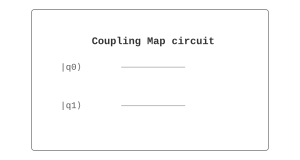
\includegraphics[width=0.6\textwidth]{../../images/coupling_map_circuit.svg}
\end{center}

\subsection{数学推导}

耦合映射：
\begin{equation}
G = (V, E)
\end{equation}

其中 $V$ 是量子比特集合，$E$ 是连接边集合。

\subsection{几何解释}

耦合映射描述量子硬件的连接拓扑。只有相邻的量子比特才能直接执行双量子比特门。

\section{代码详解}

\begin{verbatim}
from quonic.compile import coupling_map

# coupling_map(backend)
# backend: 后端名称

cm = coupling_map(backend='ibmq_manila')

# cm: 耦合映射
# cm.nodes: 量子比特
# cm.edges: 连接边
print(f'Coupling map: {cm}')
\end{verbatim}

\section{进阶用法}

\subsection{场景 1：不同后端}

\begin{verbatim}
from quonic.compile import coupling_map

# 不同后端
cm1 = coupling_map(backend='ibmq_manila')
cm2 = coupling_map(backend='ibmq_quito')
cm3 = coupling_map(backend='ibmq_belem')
\end{verbatim}

\section{适用场景}

\subsection{量子编译}

耦合映射用于量子编译器，将逻辑电路映射到物理硬件。

\subsection{硬件优化}

耦合映射用于优化量子硬件的连接拓扑。

\section{常见问题}

\subsection{耦合映射和量子硬件有什么关系？}

耦合映射描述量子硬件的连接拓扑。只有相邻的量子比特才能直接执行双量子比特门。

\subsection{如何选择耦合映射？}

选择耦合映射需要考虑硬件特性、电路需求等因素。

\section{学习路径}

\subsection{前置知识}
\begin{itemize}
  \item 量子硬件
  \item 量子门
  \item 图论
\end{itemize}

\subsection{继续学习}
\begin{itemize}
  \item 量子编译
  \item 电路映射
  \item 量子硬件优化
\end{itemize}

\section{完整示例代码}

\subsection{示例 1：基本耦合映射}

\begin{verbatim}
from quonic.compile import coupling_map

cm = coupling_map(backend='ibmq_manila')
print(f'Coupling map: {cm}')
\end{verbatim}

\section{下载}

\begin{itemize}
  \item [coupling\_map.py](https://github.com/ChrisLee0721/QuoNic/blob/main/examples/coupling_map/coupling_map.py)
\end{itemize}

\end{document}
